\documentclass[oneside,14pt]{extarticle}
\usepackage[utf8]{inputenc}
\usepackage[english,ukrainian]{babel}
\usepackage{amssymb,amsfonts,amsmath,amsthm,mathtext,textcomp}

\usepackage[includehead, headsep=0pt, footskip=0pt, top=2cm, bottom=2cm, left=2cm, right=1cm]{geometry}
\usepackage{indentfirst}
\usepackage[onehalfspacing]{setspace}
\usepackage[headings]{fancyhdr}
\usepackage{etoolbox}
\usepackage{flafter}
\usepackage{listings}
\usepackage{graphicx}
\usepackage{float}
\usepackage[labelsep=period]{caption}
\lstset{
	breaklines=false
}
\usepackage{array}
\fancyhf{}
\renewcommand{\headrulewidth}{0pt}
\pagestyle{fancy}
\fancyfoot[R]{\thepage}
\lstset{breaklines=true,}
\graphicspath{ {./pictures} }

\lstset{
	language=c,
	tabsize=4,
	keepspaces,
	showstringspaces=false,
}
\graphicspath{ {./pictures} }
\setlength{\parindent}{4em}
\setlength\tabcolsep{5px}

\newcommand\subject{Моделювання та аналіз програмного забезпечення}
\newcommand\lecturer{доцент кафедри ПЗ \\ Сердюк П.В.}
\newcommand\teacher{викладач кафедри ПЗ \\ Микуляк А.В.}
\newcommand\mygroup{ПЗ-22}
\newcommand\lab{6}
\newcommand\theme{Дослідження предметної області та
	проектування системи за допомогою UML діаграм}
\newcommand\purpose{Дослідити предметну область та
	проектування системи за допомогою UML діаграм}

\begin{document}
\begin{normalsize}
	\begin{titlepage}
		\thispagestyle{empty}
		\begin{center}
			\textbf{МІНІСТЕРСТВО ОСВІТИ І НАУКИ УКРАЇНИ\\
				НАЦІОНАЛЬНИЙ УНІВЕРСИТЕТ "ЛЬВІВСЬКА ПОЛІТЕХНІКА"}
		\end{center}
		\begin{flushright}
			\textbf{ІКНІ}\\
			Кафедра \textbf{ПЗ}
		\end{flushright}
		\vspace{70pt}
		\begin{center}
			\textbf{ЗВІТ}\\
			до лабораторної роботи № \lab\\
			\textbf{на тему}: “\textit{\theme}”\\
			\textbf{з дисципліни}: “\subject”
		\end{center}
		\vspace{50pt}
		\begin{flushright}
			
			\textbf{Лектор}:\\
			\lecturer\\
			\vspace{10pt}
			\textbf{Виконав}:\\
			
			студент групи \mygroup\\
			Коваленко Д.М.\\
			\vspace{10pt}
			\textbf{Прийняв}:\\
			
			\teacher\\
			
			\vspace{28pt}
			«\rule{1cm}{0.15mm}» \rule{1.5cm}{0.15mm} 2023 р.\\
			$\sum$ = \rule{1cm}{0.15mm}……………\\
			
		\end{flushright}
		\vspace{\fill}
		\begin{center}
			\textbf{Львів — 2023}
		\end{center}
	\end{titlepage}
		
	\begin{description}
		\item[Тема.] \theme.
		\item[Мета.] \purpose.
	\end{description}

	\section*{Завдання}
Відповідно до завдання, яке ви виконуєте у рамках команди (3-4 студенти в команді)
розробити:
\begin{itemize}
	\item діаграму діяльності;
	\item діаграму класів (+- 10 класів для кожного студента).
\end{itemize}

Врахувати у проектах інтерактивну взаємодію користувачів. Всі діаграми повинні бути
складними, оскільки кінцевої реалізації проекту не потрібно, як і всіх задекларованих
можливостей у діаграмах.

Побудувати діаграму класів із використанням основних парадигм ООП. Для інкапсуляції
логіки, створити щонайменше 2 модулі: модуль з класами, що відповідальні за внутрішню
логіку програми (бізнес-логіку) та модуль інтерфейсу користувача. Модифікатори доступу
класів і полів повинні надавати доступ лише до необхідних елементів, усі решта повинні бути
невидимі розробнику інтерфейсу користувача.

Ролі у команді - TL:
\begin{itemize}
	\item Розробити діаграми компонент і розгортання. Спроектувати збірки: моделі,
	Unit тести, клієнта з графічним інтерфейсом (web, mobile, desktop). Якщо є
	необхідність то реалізувати інші збірки: сервера, іншого клієнт (наприклад
	може бути 2 клієнта – під веб та під мобільний пристрій).
\end{itemize}
	\section*{Хід виконання}
	\begin{figure}[H]
		\centering
		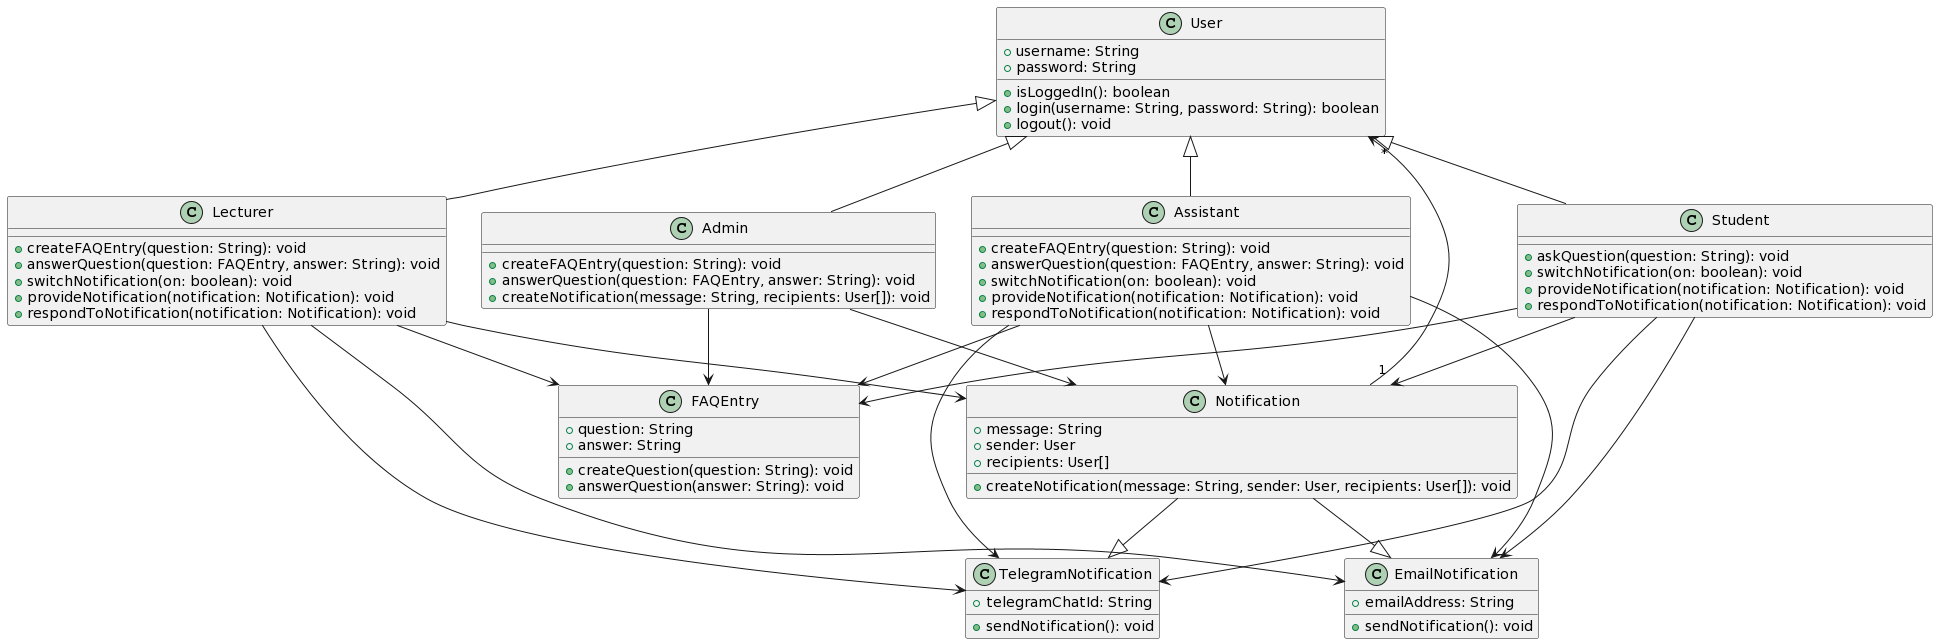
\includegraphics[width=\textwidth]{class}
		\caption{Діаграма класів виконанана відповідно до індивідуального варіанту}
	\end{figure}
	
	\begin{figure}[H]
		\centering
		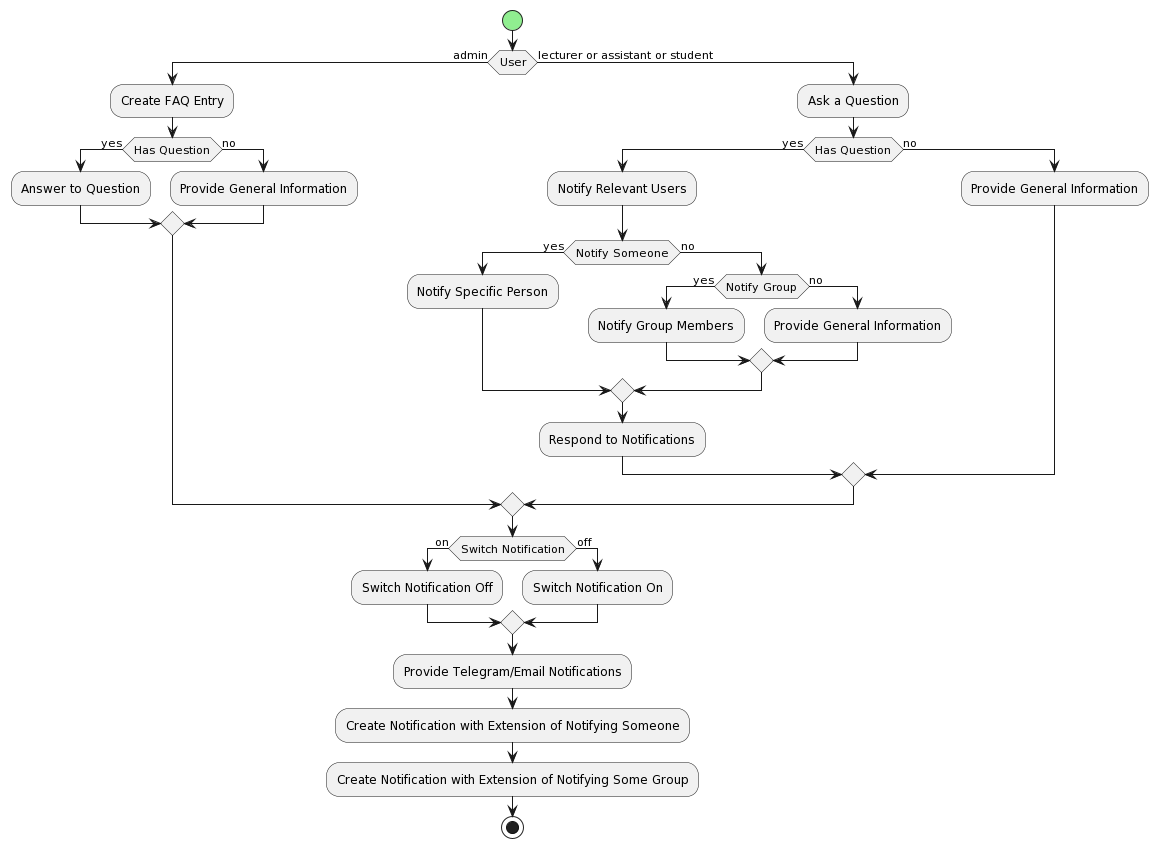
\includegraphics[width=\textwidth]{activity}
		\caption{Діаграма діяльності виконана відповідно до індивідуального варіанту}
	\end{figure}
	
	\begin{figure}[H]
		\centering
		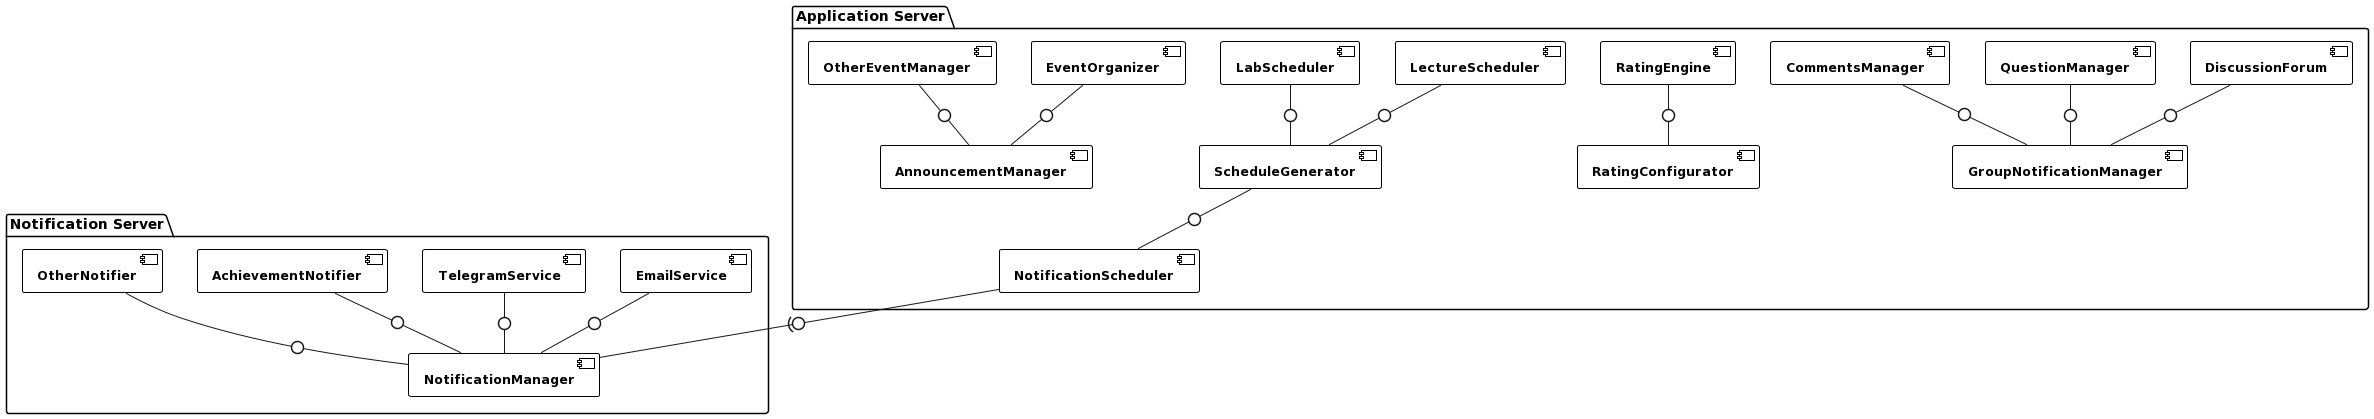
\includegraphics[width=\textwidth]{component}
		\caption{Діаграма компонентів виконана відповідно до ролі у команді}
	\end{figure}
	
	\begin{figure}[H]
		\centering
		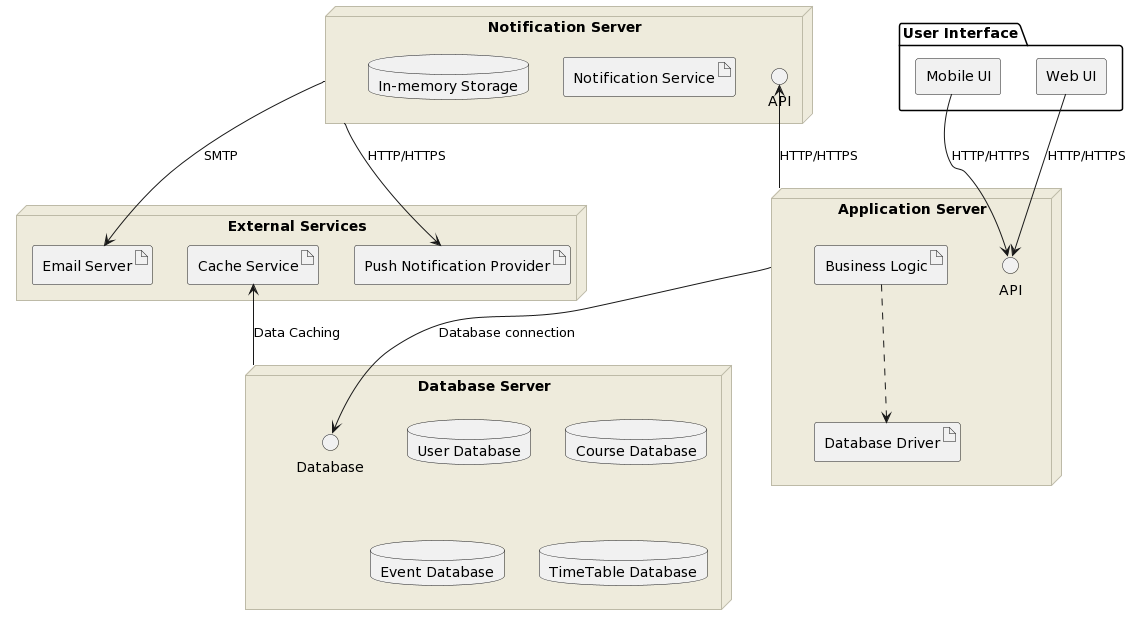
\includegraphics[width=\textwidth]{deployment}
		\caption{Діаграма розгортання виконана відповідно до ролі у команді}
	\end{figure}
	
	\begin{figure}[H]
		\centering
		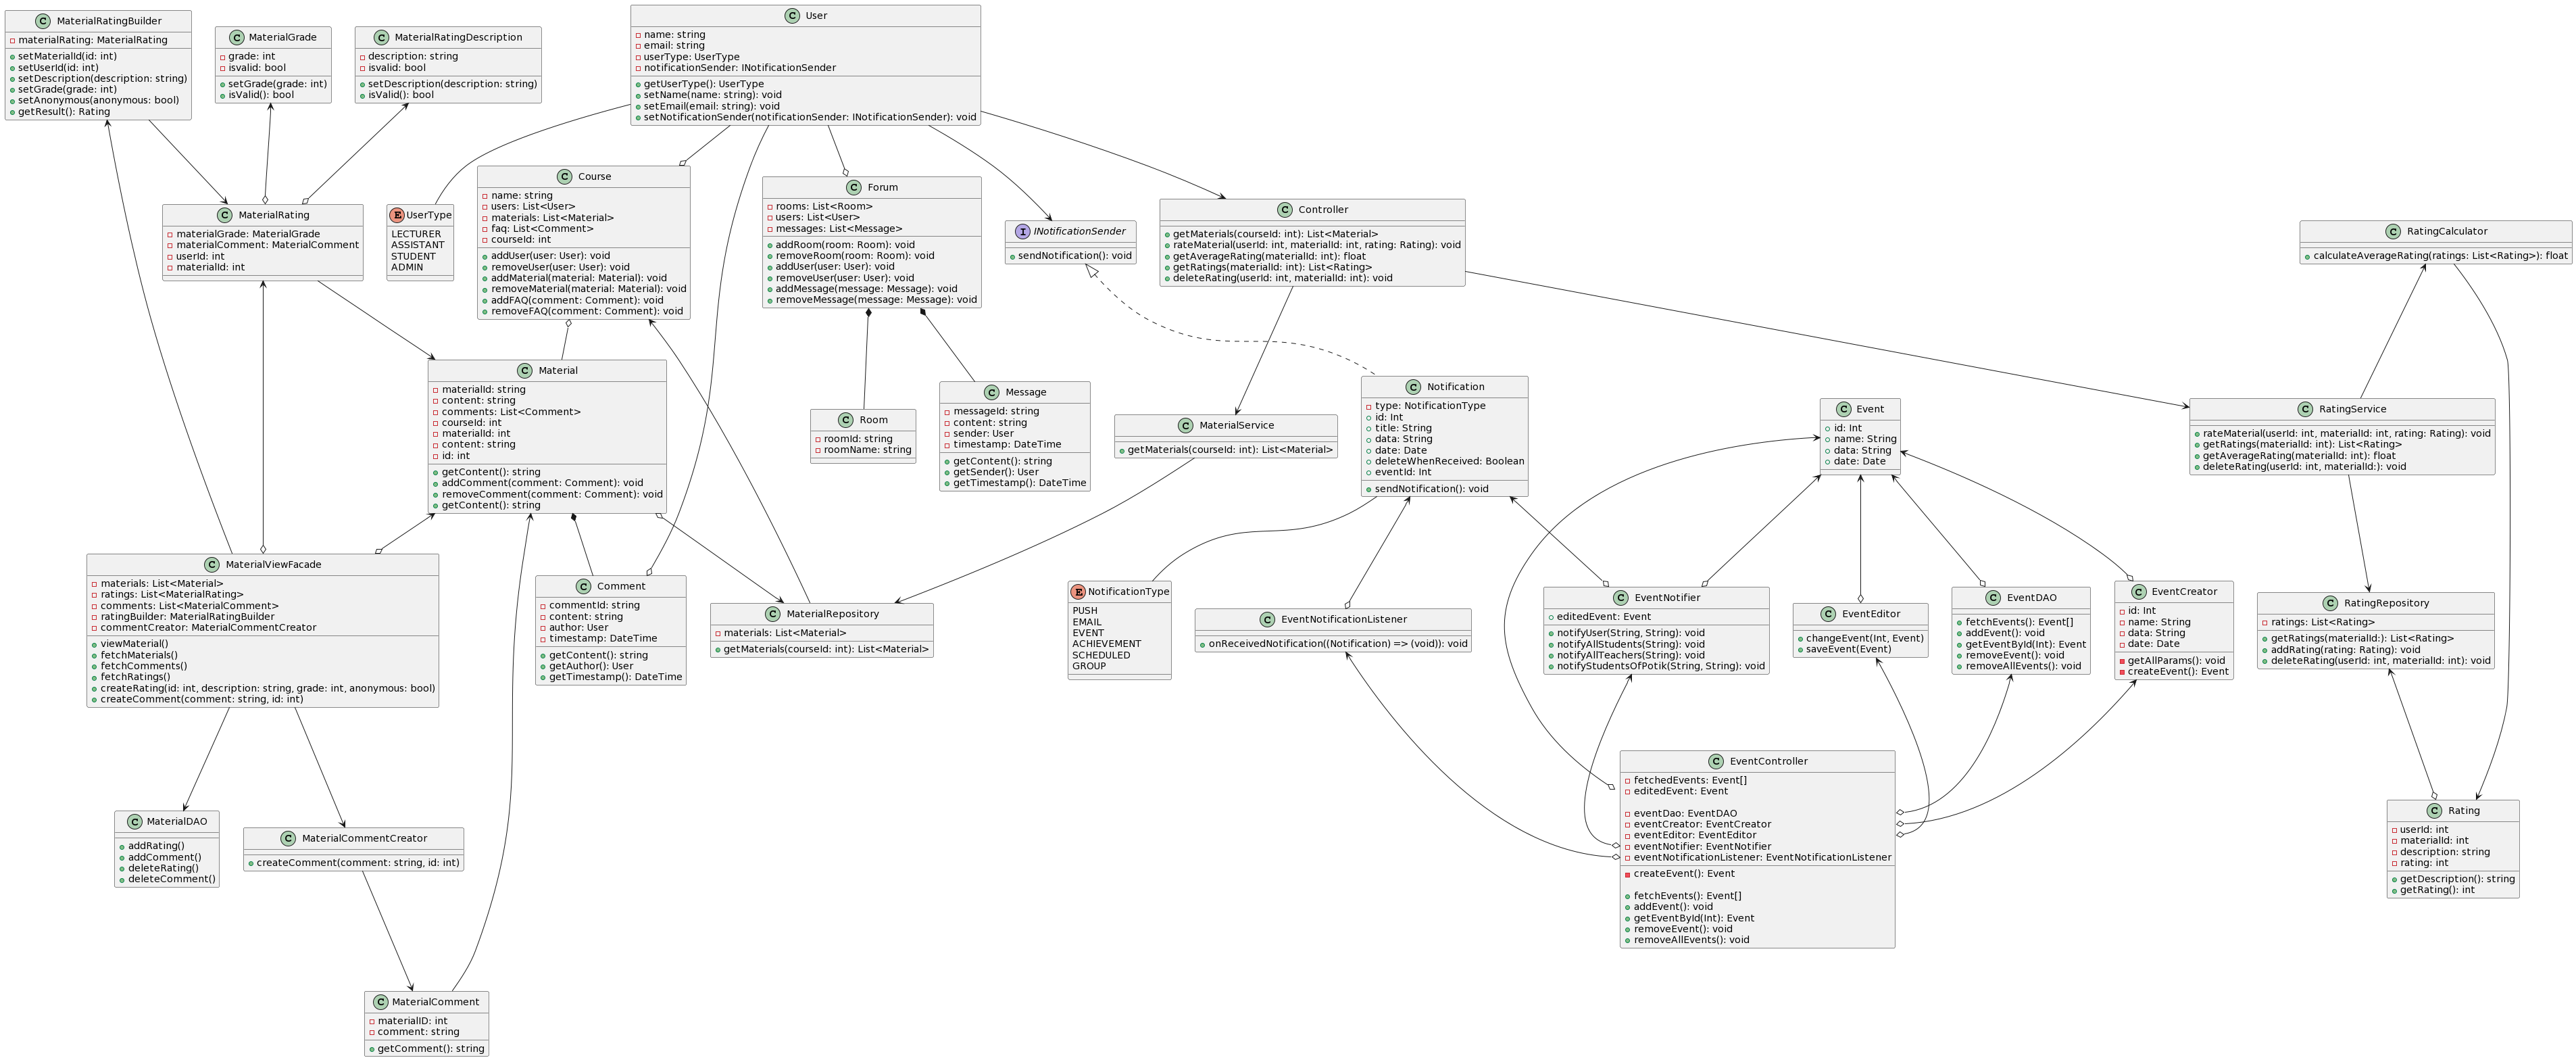
\includegraphics[width=\textwidth]{classes}
		\caption{Діаграма класів виконана відповідно до ролі у команді}
	\end{figure}
		
	\section*{Проектування збірок системи}
	\subsection*{Створення моделей}
		
    Використати популярні фреймворки машинного навчання TensorFlow та PyTorch, для розробки та навчання необхідних моделей.
Використовувати мову програмування Python для розробки моделей та створити конфігурацію збірки, що включає необхідні залежності та інструменти.
Реалізувати модульні тести для перевірки точності та функціональності моделей.
	
\subsection*{Створення модульних тестів}
	
    Обрати фреймворк для тестування, такий як pytest або JUnit, для написання модульних тестів для різних компонентів системи.
Налаштувати конфігурацію збірки для компіляції та виконання модульних тестів, забезпечивши повне охоплення критичної функціональності.
Використовувати інструменти, такі як Mockito або TestNG, для створення підробок і підмінних об'єктів під час модульного тестування.
	
\subsection*{Створення веб-користувацького інтерфейсу (UI)}
	
    Для веб-інтерфейсу використовувати сучасні технології веб-розробки, такі як React.js або Angular.
Використовувати HTML5, CSS3 та JavaScript для створення інтерактивного та адаптивного веб-інтерфейсу.
Використовувати інструменти збирання, такі як Webpack або Babel, для пакування та оптимізації коду веб-інтерфейсу.
Включити фреймворки, такі як Jest або Enzyme, для модульного тестування компонентів веб-інтерфейсу.
	
\subsection*{Створення мобільного інтерфейсу (UI)}
	
    Вибрати кросплатформенний фреймворк для розробки мобільного інтерфейсу, такий як React Native або Flutter.
Розробити мобільний інтерфейс з використанням вибраного фреймворку, що дозволяє використовувати спільний код для кількох платформ.
Використовувати інструменти, такі як Expo або Android Studio, для збирання та упаковки мобільного додатка.
Проводити модульне тестування мобільного інтерфейсу за допомогою інструментів, таких як Jest або вбудований фреймворк тестування Flutter.
	
\subsection*{Розгортання та інтеграція}
	
    Розгорнути артефакти веб-інтерфейсу на веб-сервері або хмарній платформі AWS.
Упакувати мобільний додаток для розповсюдження через магазини додатків, такі як Google Play та Apple App Store.
Налаштувати сервер додатка для виконання бізнес-логіки, використовуючи API через RESTful-точки доступу по протоколу HTTP та HTTPS.
Встановити з'єднання між сервером додатка та сервером бази даних за допомогою ORM-фреймворку, такого як Hibernate.
Налаштувати сервер кешування для можливості кешування даних, використовуючи технології, такі як Redis або Memcached.
Інтегрувати сервер сповіщень з електронною поштою за допомогою протоколів SMTP та підключитися до зовнішніх провайдерів сповіщень через їхні API.


	\section*{Висновки}
	   Під час виконання лабораторної роботи мною був проведений детальний аналіз предметної області та розроблена система за допомогою UML діаграм. Цей процес дозволив мені зрозуміти вимоги до системи, її функціональність та структуру. 
	   
	   Я отримав складні діаграми, що демонструють структуру та логіку проекту, зокрема взаємодію з користувачами. Це допомагло команді розуміти вимоги та функціональні можливості системи, а також сприяло подальшій розробці та розгортанню проекту.
\end{normalsize}
\end{document}
